В том случае, если рентгеновское излучение отражается от атомных плоскостей, не
 параллельных поверхности, говорят об асимметрии отражения (рис. \ref{ris:assymetric_brag}).

Для того чтобы охарактеризовать степень асимметрии, вводят коэффициент $b$:

\begin{equation}
  b = \frac {\gamma_0}{|\gamma_h|}
  \label{eq:koef_b}
 \end{equation}

\noindent
где, $\gamma_0 = cos \psi_0 = sin ( \varphi + \theta_B)$, $\gamma_h = cos \psi_h = sin ( \varphi - \theta_B)$,
$\varphi$ - угол между плоскостью отражения и поверхностью образца. Данный коэффициент, как будет показано дальше,
может существенным образом влиять на картину дифракции.

\begin{figure}[H]
  \centering
  \subfloat[]{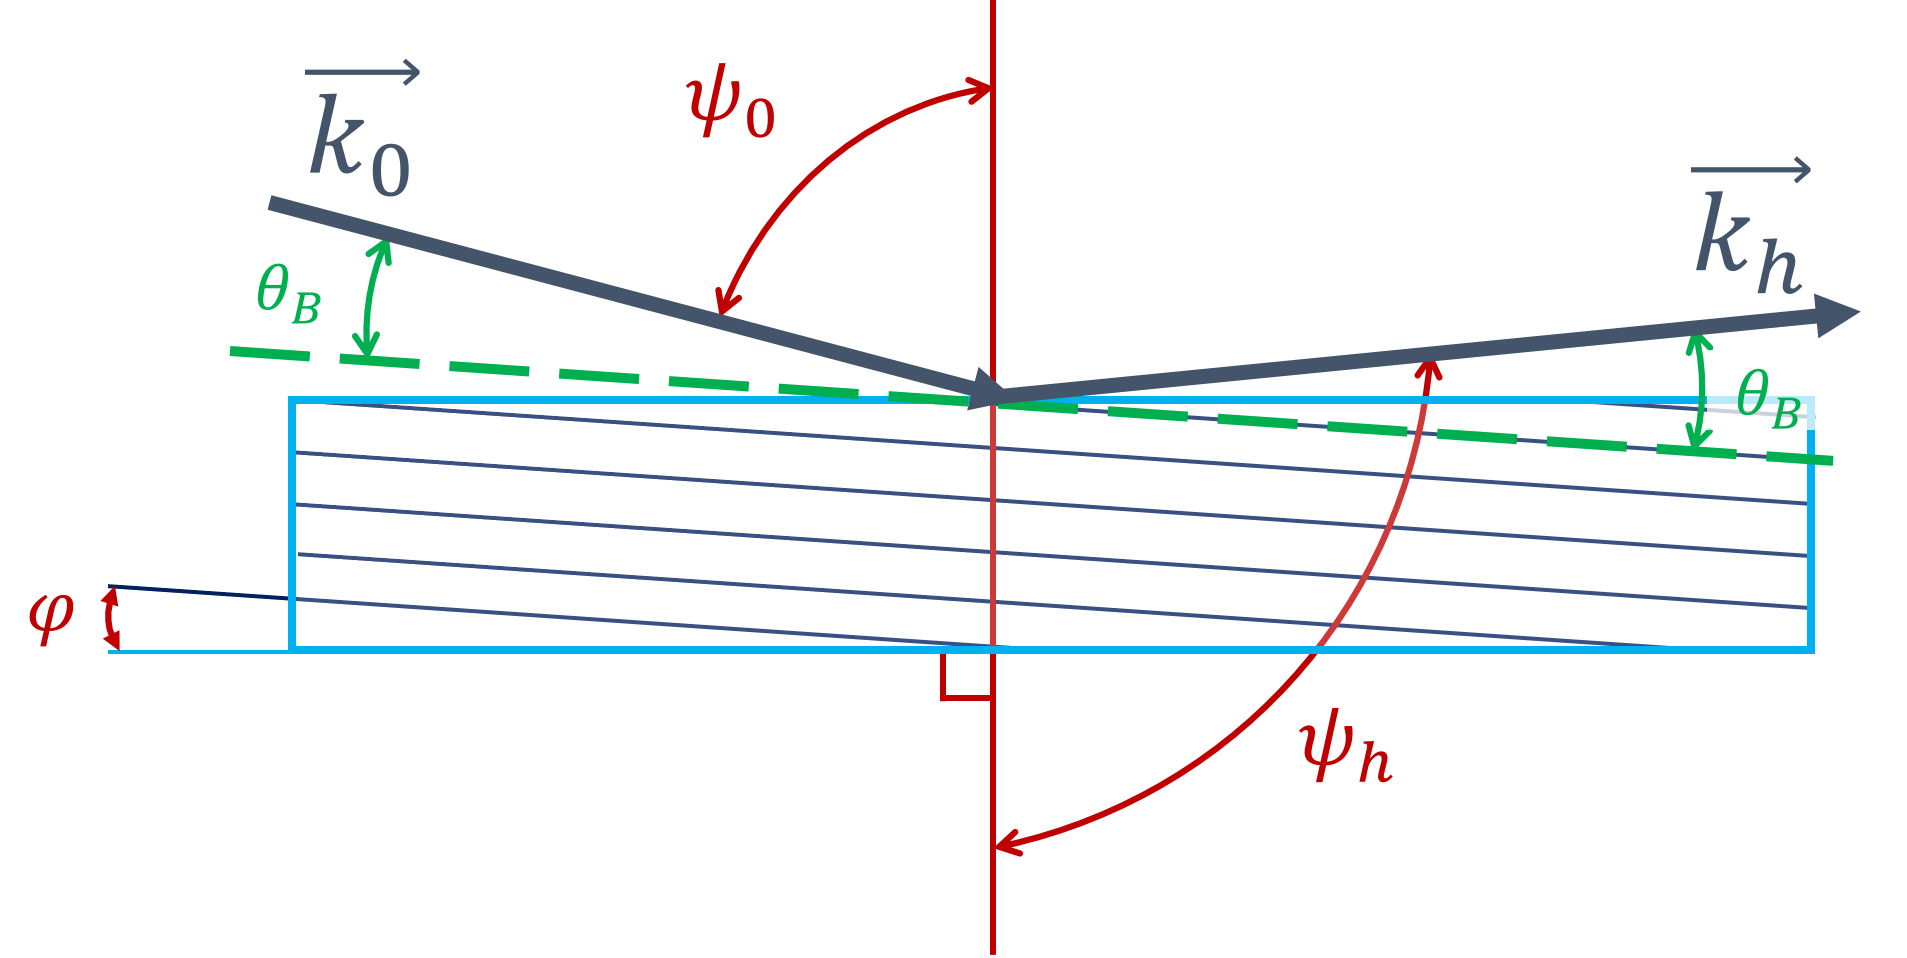
\includegraphics[width=0.45\textwidth]{images/assym2.png}}
  \hfill
  \subfloat[]{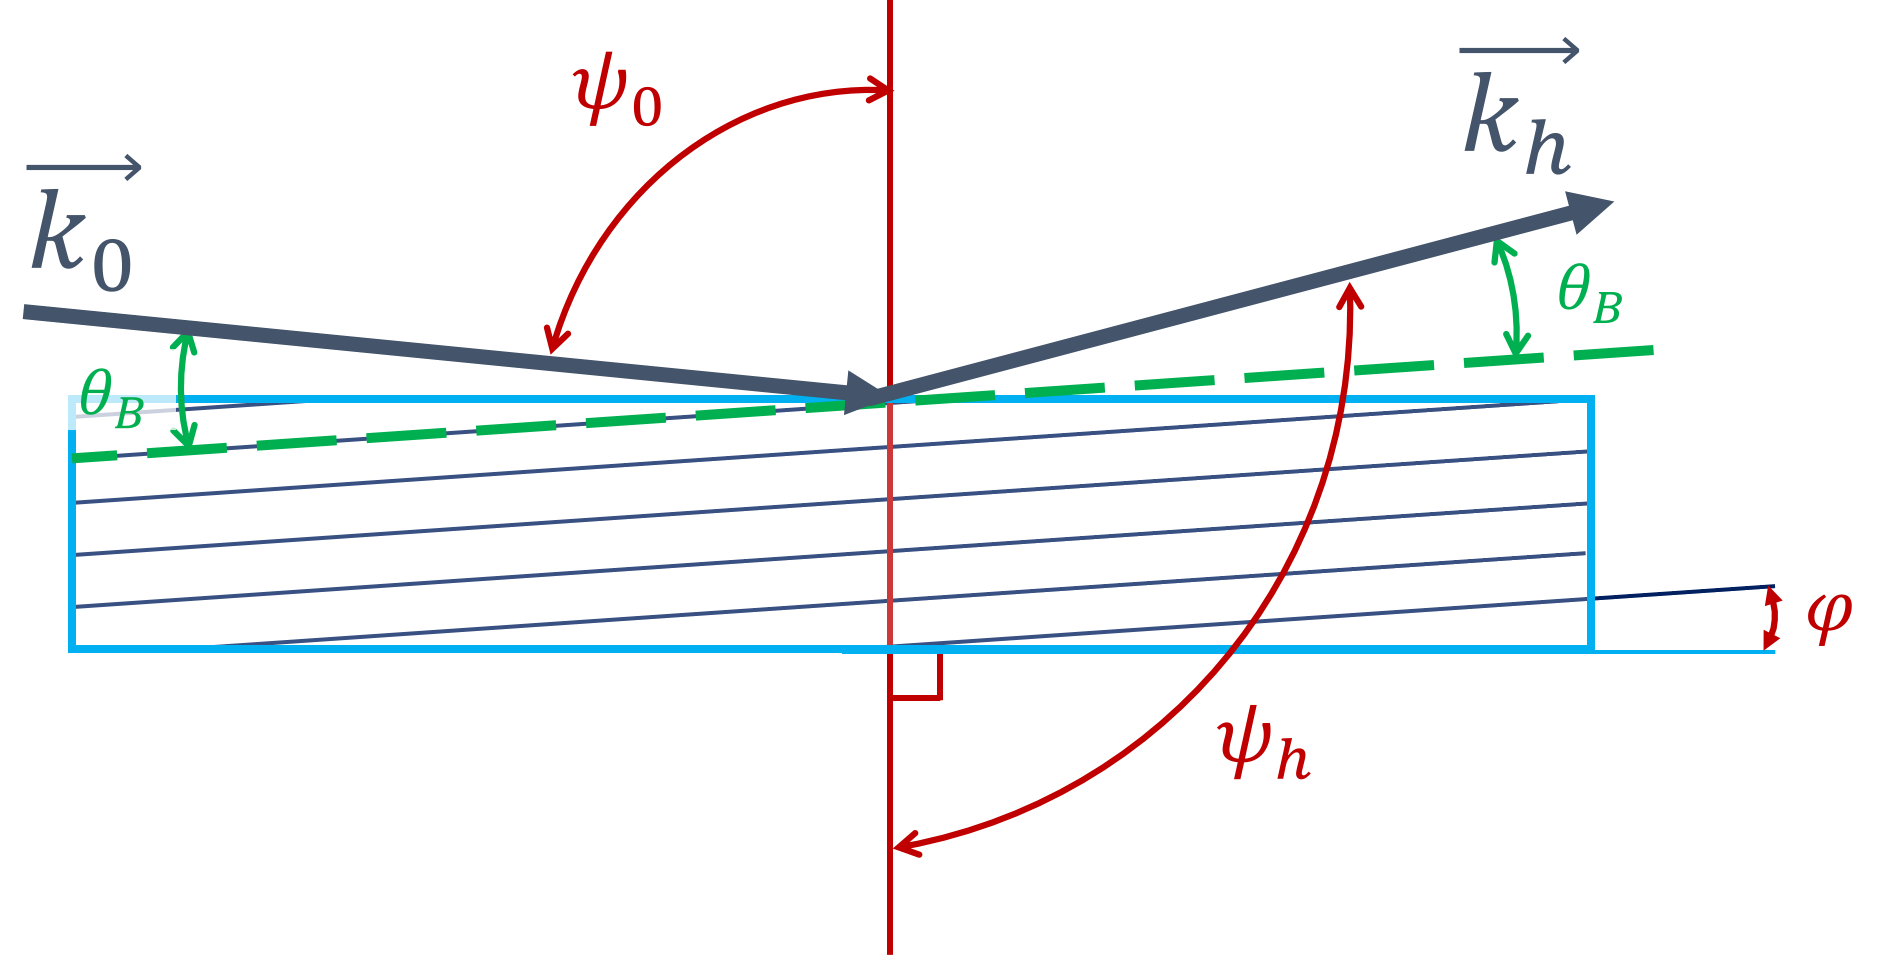
\includegraphics[width=0.45\textwidth]{images/assym1.png}}
  \caption{Схема асимметричной брэгговской дифракции для коэффициента  $b >> 1$; $\varphi$ > 0 (a),
   $b << 1$; $\varphi$ < 0 (b)}
  \label{ris:assymetric_brag}
\end{figure}
